\section{Introduction}

\if 0

%% Intro outline

Many new proposals for congestion control: see timeline figure. Today, to deploy, needs to be in TCP in the kernel --> , along with which datapath platforms (to our knowledge) have which algorithms. A new congestion control algorithm involves kernel development, but equally important, upstreaming and maintenance. --> is that true? Can't we develop and install kernel module congestion control methods using the pluggable TCP API?

Many datapaths now being used, and more promise to come (e.g., hardware); generally, they lack rich cc algorithms. Because they often bypass the kernel, don't use TCP, or both, there is a significant development effort.

The "cross product" of algorithms X datapaths is large.

Our goals: 

1. write once, run anywhere
2. increase "velocity" of development;build cc algorithms in a modular way from components. Demonstrate fidelity, i.e., accuracy wrt an in-datapath impl
3. enable new capabilities and algorithms, e.g., aggregation. 

\fi

Due to the continual deployment of new applications and network technologies, and changes in workload patterns, research on congestion control has not only remained vibrant since the 1980s, but has flourished in recent years. Figure~\ref{fig:cctimeline} shows a time-line of innovations in this area. 

\begin{figure}[t]
\centering
    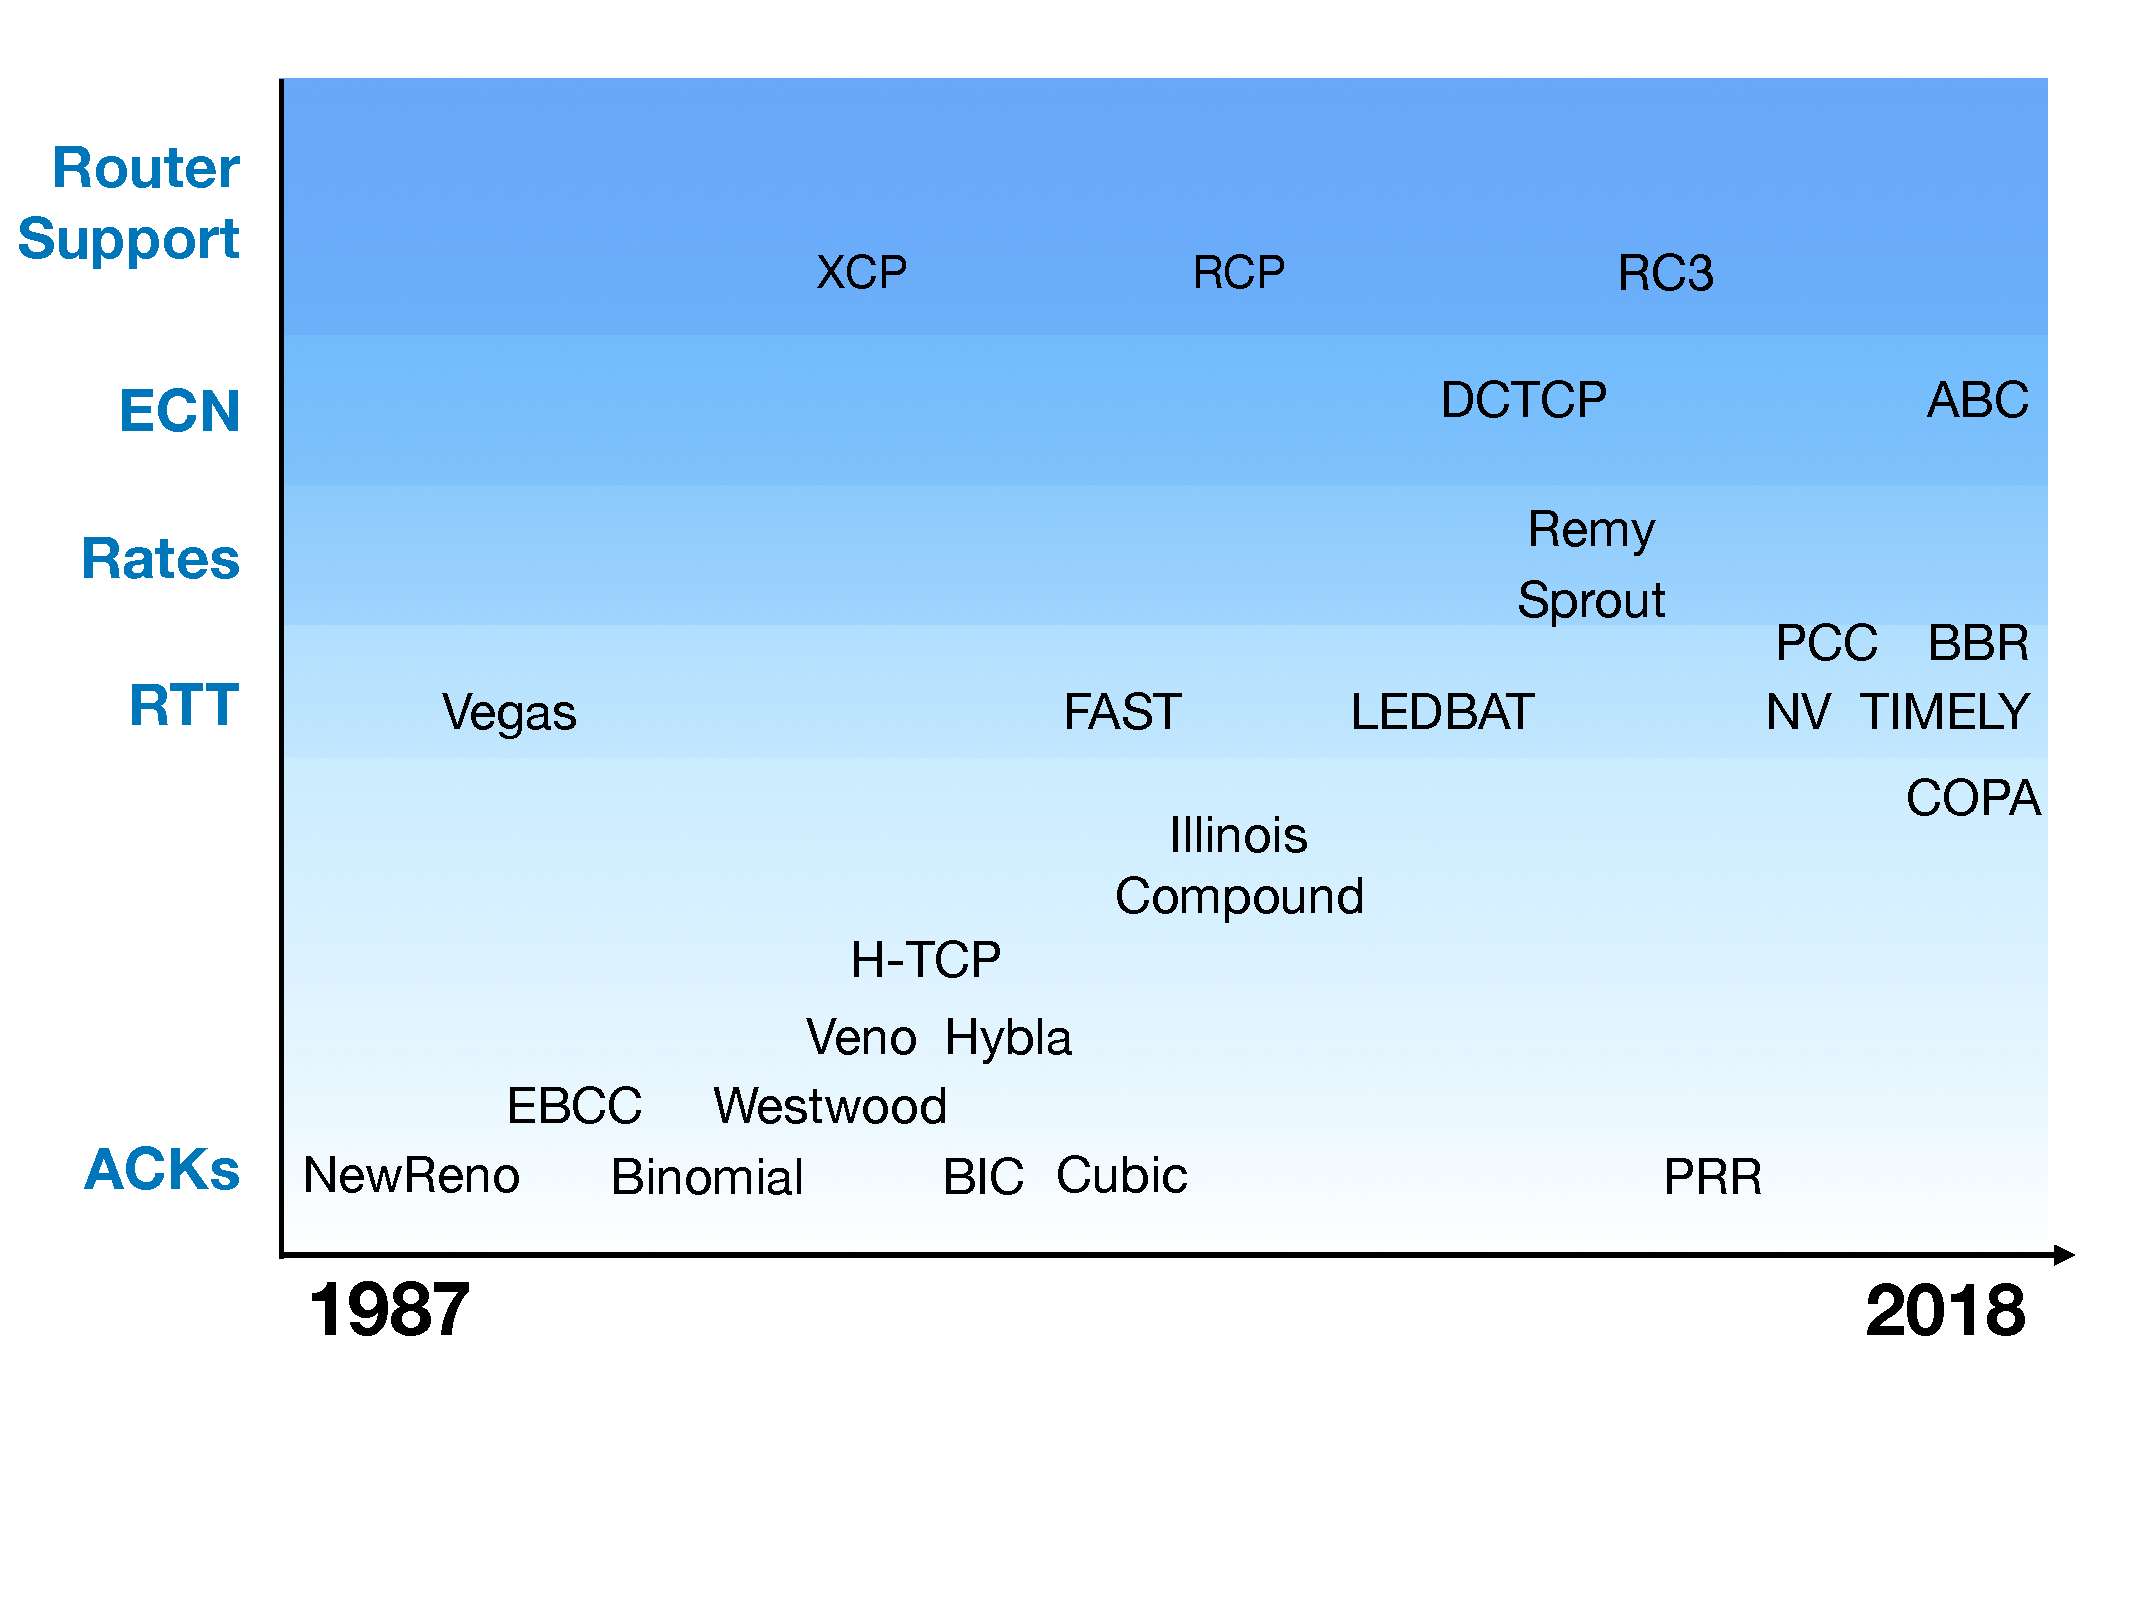
\includegraphics[width=\columnwidth]{img/cc-timeline}
    \vspace{-1cm}
    \caption{As link characteristics diversify, a developers have developed a battery of congestion control algorithms, from the ``long-fat pipe'' schemes of the mid-2000s~\cite{westwood, veno, htcp, hybla} to purely delay-based~\cite{vegas, fasttcp, ledbat, nv, timely} and hybrid loss-delay~\cite{illinois, compound} schemes, and more recent proposals~\cite{pcc, remy, sprout, bbr, copa, abc}.}\label{fig:cctimeline}
\end{figure}

At its core, a congestion control protocol determines when each segment of data must be sent. Because a natural place to make this decision is within the transport layer, congestion control today is tightly woven into kernel TCP software and runs independently on each TCP connection.

An operating system's TCP software is but one example of a {\em datapath}, the term we use for any module that provides data transmission and reception interfaces between higher-layer applications and lower-layer network hardware. Recently, many other datapaths have emerged, including user-space protocols atop UDP (e.g., QUIC~\cite{quic}, WebRTC~\cite{webrtc}, Mosh~\cite{mosh}), kernel-bypass methods (e.g., mTCP/DPDK~\cite{dpdk,mtcp,netmap}), RDMA~\cite{dcqcn}, multi-path TCP (MPTCP)~\cite{mptcp}, and specialized Network Interface Cards (``SmartNICs''~\cite{smartnic}). This trend suggests that the future will likely see many applications using datapaths different from kernel-supported TCP connections.

New datapaths typically do not offer much in terms of congestion control because implementing these algorithms correctly takes considerable time and effort. For instance, the set of available algorithms in mTCP~\cite{mtcp}, a TCP implementation on DPDK, is limited to a variant of Reno. Lest one dismiss this example as a case of a research project lacking in engineering resources, we note that QUIC, despite Google's imposing engineering resources, does not have most of the algorithms that have been implemented in the Linux kernel over many years.  We expect this situation to worsen with the emergence of new hardware accelerators and programmable network interface cards (NICs) because high-speed hardware designers tend to forego programming convenience for performance. The difficulty isn't the volume of code, but the many subtle correctness and performance issues in various algorithms that are tricky, requiring expertise to understand and resolve.

This paper starts from the observation, made in a recent position paper~\cite{ccp-hotnets}, that congestion control algorithms do not need to be implemented in the datapath. If the datapath encapsulated the information available to it about {\em congestion signals} like the round-trip time (RTT), packets received and lost, explicit congestion notification (ECN) markings, etc., and periodically provided this information via a well-defined interface to an off-datapath module, then congestion control algorithms could run in the context of that module. Then, by exposing an analogous interface to control transmission parameters such as the window size, pacing rate, and transmission pattern, the datapath could transmit data according to the policies of the off-datapath congestion control algorithm. 

%The off-datapath congestion control algorithm can then control the transmission parameters of the datapath such as the window size, pacing rate, and transmission pattern via an analagous {\em control interface} provided by the datapath.

We use the term {\em Congestion Control Plane (CCP)} to refer to this off-datapath module. Running congestion control in the CCP offers the following benefits:
\begin{enumerate}
    \item {\bf Write-once, run-anywhere:} With CCP, one can write a congestion control algorithm once and run it on any datapath that supports the specified interface. We demonstrate in this paper a variety of algorithms running on three datapaths: the Linux kernel, mTCP/DPDK, and QUIC, and show algorithms running for the first time on certain datapaths (e.g., Cubic on mTCP/DPDK, Copa on QUIC).
    % MA: I removed Reno on mTCP, because we said eariler that dpdk has some variant of Reno
    
    \item {\bf Higher ``velocity'' of development:} With the right abstractions, a congestion control designer can focus on the algorithmic essentials without worrying about the details and data structures of the datapath. The result is more expressive, easier to maintain code. We show a deployment mode where CCP and the algorithms run at user level, which means that new algorithms can be deployed in production without the cumbersome ``upstreaming'' process. (Of course, the modifications we propose to the datapath must be deployed and upstreamed, but that effort does not grow with the number of algorithms).
    %CCP also provides reusable modules for commonly used congestion control components such as multiplicative increase, additive increase, multiplicative decrease, etc., and allows us to write algorithms not tied to the ACK clock (i.e., it is easier to express methods such as equation-based control that update rates at times unrelated to ACK arrivals).
    % MA: The reusable modules point feels weaker than our other benefits. A possible reaction is: how hard is it to implement things like AI, MI, MD, anyway? Isn't it a few lines of code? Are there better examples of modules?
    
    \item {\bf New capabilities:} CCP makes it easier to provide new capabilities, such as aggregate control of multiple flows as previously proposed in the congestion manager~\cite{cm}, and writing and debugging new algorithms that require significant computation (e.g., signal processing, machine learning, etc.).
\end{enumerate}

Our design and implementation of CCP includes the following contributions: 
%\hb{Weave in performance numbers into these items as needed}

\begin{itemize}
\item A flexible API to request measurements from and exercise control over the datapath (\S\ref{s:design}). We define a small language with which algorithms can specify custom summaries over per-packet information. 
%fold functions and control patterns to exercise control over datapath behavior from a CCP program (algorithm)

\item A specification of datapath responsibilities (\S\ref{s:datapath}). These include congestion signals that a datapath should maintain, as well as a simple framework to execute directives from a CCP program. This design enables ``write-once, run-anywhere'' protocols. We demonstrate this capability with several examples, showing multiple cases of the same CCP algorithm code running over three different datapaths. 

\item An exploration of the design space of new capabilities enabled by CCP (\S\ref{sec:ccp}): the rapid development of new algorithms and implementing an aggregate congestion controller.

\item A demonstration of the fidelity of CCP in a variety of link conditions. Our CCP implementation matches the performance of Linux kernel implementations at only a small overhead (5\% more CPU utilization in the worst case). Furthermore, we show it is feasible to implement infrequent congestion control even in low-RTT, high bandwidth environments.

\end{itemize}


% 1. APIs for programmatic control of measurement and packet transmission functions. The challenge is to identify general primitives that can express a broad range of congestion control algorithm and can be supported by a variety of datapaths. Give examples. We can mention something about our streaming schema, control patterns, etc. here.
% 2. A language and simple instruction set for expressing stateful summaries (e.g., moving average of RTT measurements)  in the datapath. By supporting in-datapath summaries, we enable usecases where CCP-datapath communication is expensive. For example, a userspace CCP can control the Linux kernel TCP datapath based on periodic updates (e.g., every 10 ms), and yet retain fine-grained visibility into per-packet congestion signals.  
%\if 0
%
%We have implemented an example CCP as a user-level Linux program and have run experiments with many congestion control algorithms in CCP over three different datapaths. Our results show that
%
%\begin{enumerate}
%    \item 
%    
%    \item 
%    
%    \item 
%    
%\end{enumerate}
%
%\fi
%
%
%
%